\section{Evaluation}
\label{sec:evalation}

In this section, we evaluate SpryVM with conventional translation using $4$KB and $2$MB pages, and qualitatively with the other prior work.   

\begin{figure*}[t]
	\centering
	\subfloat[Hash Table]{
		\label{fig:memcached_2p_assoc}
		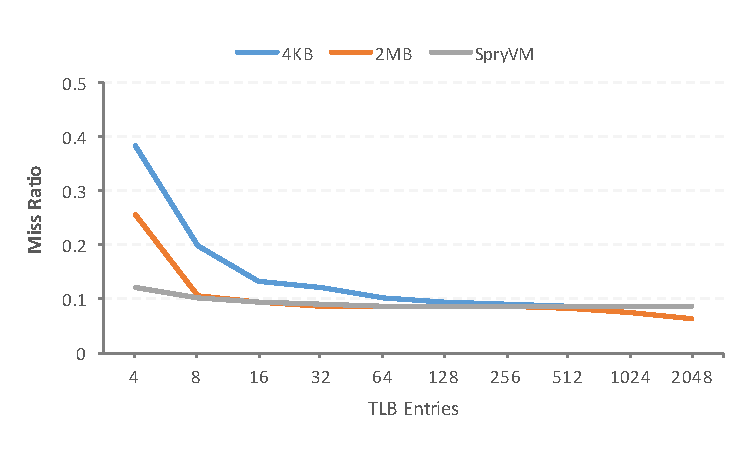
\includegraphics[width=0.3\textwidth,clip]{graphs/HT_32GB.pdf}}
	\subfloat[Skip List]{
		\label{fig:memcached_4p_assoc}
		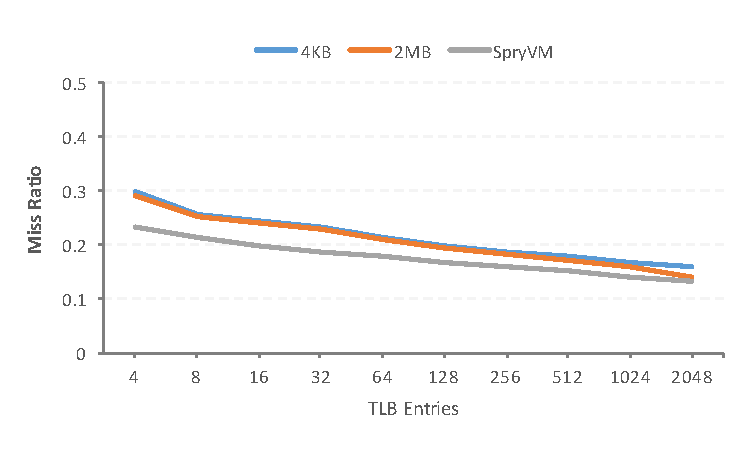
\includegraphics[width=0.3\textwidth,clip]{graphs/SL_32GB.pdf}}
	\hspace{.01in}
	\subfloat[BST Internal]{
		\label{fig:rocksdb_2p}
		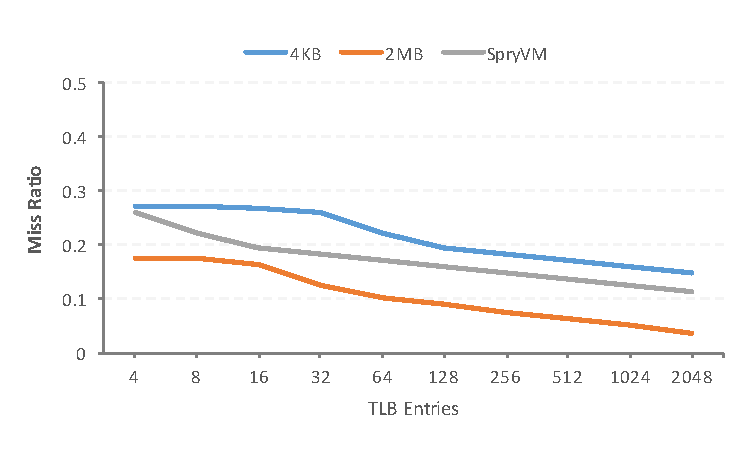
\includegraphics[width=0.3\textwidth,clip]{graphs/BSTI_32GB.pdf}}
	\subfloat[BST External]{
		\label{fig:rocksdb_4p}
		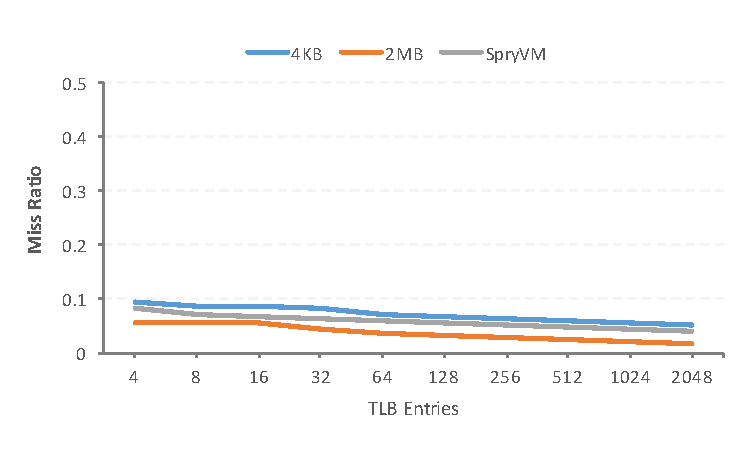
\includegraphics[width=0.3\textwidth,clip]{graphs/BSTE_32GB.pdf}}

	
	\caption{TLB sensitivity study for 32GB working set for conventional translation with 4KB and 2MB pages and SpryVM.
		\label{fig:miss_ratio_32GB}}
\end{figure*}

\begin{figure*}[t]
	\centering
	\subfloat[Hash Table]{
		\label{fig:memcached_2p_assoc}
		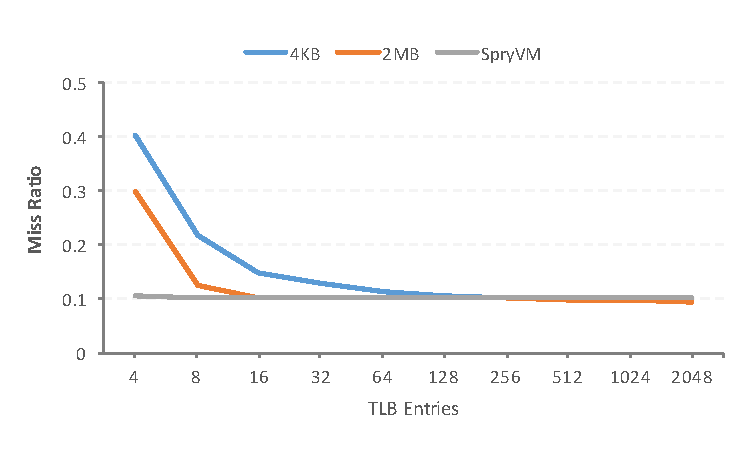
\includegraphics[width=0.3\textwidth,clip]{graphs/HT_128GB.pdf}}
	\subfloat[Skip List]{
		\label{fig:memcached_4p_assoc}
		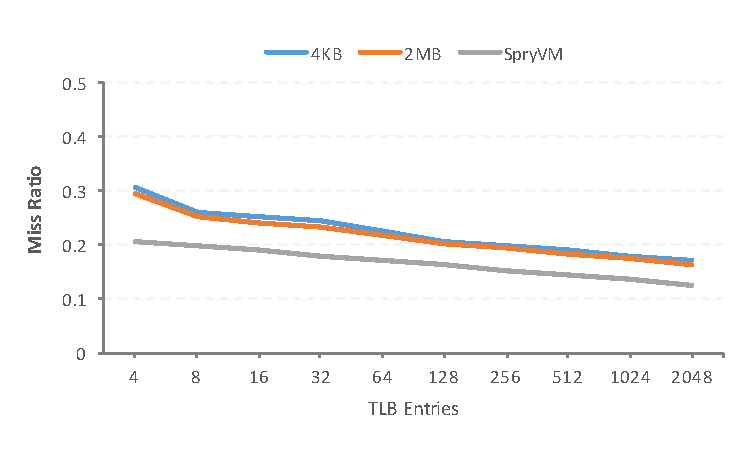
\includegraphics[width=0.3\textwidth,clip]{graphs/SL_128GB.pdf}}
	\hspace{.01in}
	\subfloat[BST Internal]{
		\label{fig:rocksdb_2p}
		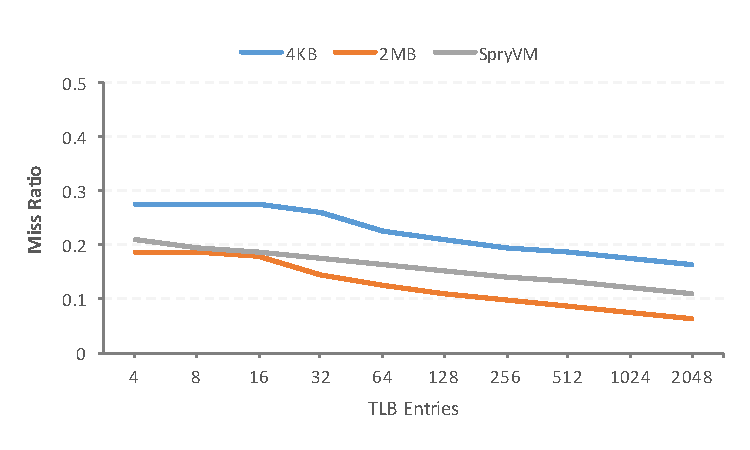
\includegraphics[width=0.3\textwidth,clip]{graphs/BSTI_128GB.pdf}}
	\subfloat[BST External]{
		\label{fig:rocksdb_4p}
		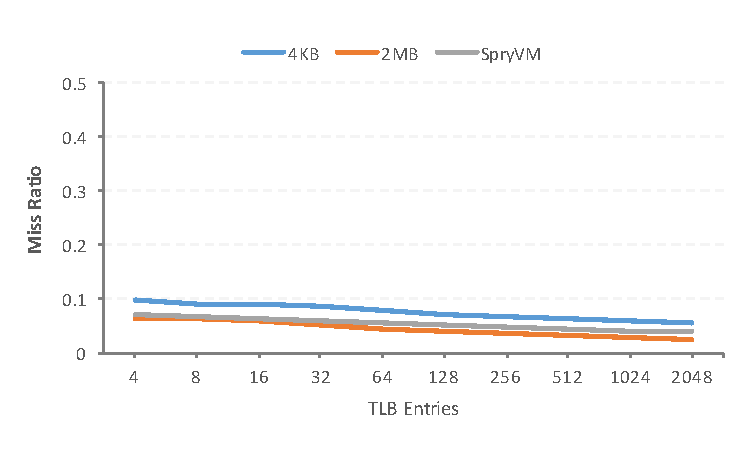
\includegraphics[width=0.3\textwidth,clip]{graphs/BSTE_128GB.pdf}}
	
	
	\caption{TLB sensitivity study for 128GB working set for conventional translation with 4KB and 2MB pages and SpryVM.
		\label{fig:miss_ratio_128GB}}
\end{figure*}

\subsection{TLB Sensitivity}

~\subsubsection{32GB working set.} Figure~\ref{fig:miss_ratio_32GB} shows the TLB miss ratio as we increase the number of entries, of the four data structure traversals, hash table, skip list, binary search tree internal, and binary search tree external, with a working set size of $32$GBs. Each graph plots three lines. The blue line represents the conventional translation mechanism using 4KB pages. The orange line the same mechanism but using $2$MB pages. The gray bar represent the TLB miss ratio of SpryVM, which uses $4$KB pages.

\noindent\textbf{4KB pages:} For all four data structures, SpryVM systematically beats conventional translation with $4$KB pages given the same TLB size. For example, for the hash table, conventional translation requires a 128-entry TLB to match the miss ratio of SpryVM with 8 entries, an $16\times$ difference. Furthermore, we see that the gap between the efficiency of TLBs worsens with the abscense of data locality. For the skip list, which is the workload with the lowest data locality, conventional translation requires around $2048$ entries to match the miss ratio of SpryVM with 16 entries.

\noindent\textbf{2MB pages:} Using $2$MB pages improves the TLB behavior of conventional translation. For example, for the hash table, with 2MB pages, conventional translation only need 8 entries to match the miss ratio of 4 entries in SpryVM, a $2\times difference$. In contrast, in workloads where there exist data locality, like in the trees, in which there is data reuse for the higher levels of the tree, the per-region $4KB$ pages are not able to beat $2$MB pages. However, note that $2$MB are not always available (as explained in the background section) and we could also employ $2MB$ pages for SpryVM; we defer that approach for future work. Furthermore, in workloads where there exists no locality, such as in the skip list data structure, $2$MB deliver an almost negligible improvement with respect to $4KB$ pages (also shown in prior work for other data structure with low data locality like graphs~\cite{haria:devirtualizing}). Hence, for the skip list, the number of TLB entries still needs to be $16\times$ bigger to match SpryVM's TLB area efficiency.

~\subsubsection{128GB working set.} Figure~\ref{fig:miss_ratio_128GB} shows the TLB miss ratio as we increase the number of entries, of the four data structure traversals with a working set size of $128$GBs. Similarly to the previous set of graphs, each graph plots three lines: the conventional translation mechanism using 4KB pages, the same mechanism but using $2$MB pages, and SryVM, which uses $4$KB pages.

\noindent\textbf{4KB pages:} For all four data structures, SpryVM systematically beats conventional translation with $4$KB pages given the same TLB size. Furthermore, the area-efficiency gap is more pronounced as the working set is larger. 

\noindent\textbf{2MB pages:} Although $2$MB pages helps to reduce the area-efficiency gap with respect to $4$KB and SpryVM, the increase in the working set worses the benefits. For example, in the hash table, $2$MB pages now requires $8\times$ the number of TLB entries to match the miss ratio of 4 TLB entries in SpryVM. Furthermore, in the cases where there is more data locality, the situation also worsens, and in fact, for the binary search tree external, now $2$MB pages and SpryVM, behave almost identically.

\subsection{TLB Miss Penalty}

\begin{figure}[t]
	\centering
	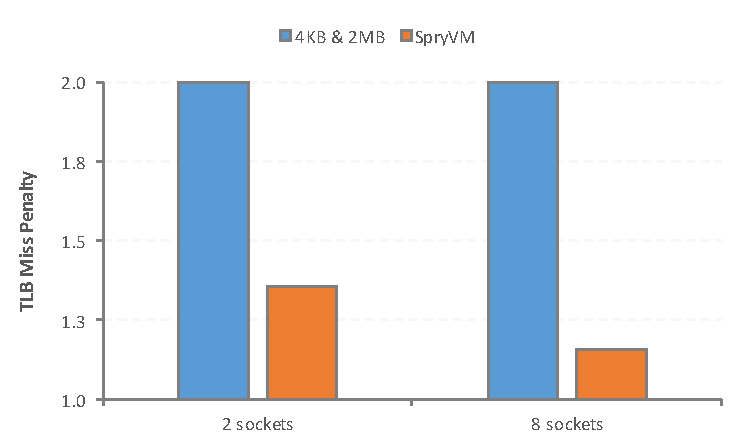
\includegraphics[width=1.0\columnwidth]{graphs/penalty.pdf}
	\caption{TLB miss penalty for conventional and SpryVM.}
	\label{fig:pagewalks}
\end{figure}